% Плоский цикл.
\subsection{Плоские циклы}

В разделах \ref{sec:text_4_small_matr} и \ref{sec:text_4_spec_matr} были рассмотрены разные варианты векторизации функций, реализующих работу с матрицами.
Эти варианты базировались на основной идее выделения однотипных операций и конструирования из них векторных аналогов.
Как видно из результатов исследований, представленных в разделах \ref{sec:text_4_small_matr} и \ref{sec:text_4_spec_matr}, эффективность векторизации сильно зависит от способа выделения таких однотипных операций, от порядка обращения в память за данными, от избыточности вычислений и других факторов.

Неоднозначность и искусственность векторизации программного кода путем поиска однотипных операций порождает потребность выработки некоторого универсального подхода к векторизации, который мог бы применяться к широкому спектру расчетных приложений.

Исследования, описанные в этом разделе, направлены на определение и описание свойств программного контекста, векторизация которого может быть выполнена достаточно прозрачно, а результирующий код будет обладать высокой степенью эффективности.

\subsubsection{Понятие плоского цикла}

Векторизация программного контекста не может быть применена автоматически к коду произвольного вида.
В данном разделе определим подходящий для векторизации программный контекст специального вида -- плоский цикл -- и опишем его свойства \cite{Shabanov2021VecCFG}.

\begin{figure}[ht]
\centering
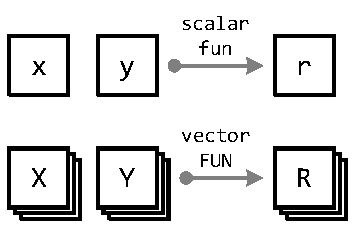
\includegraphics[width=0.4\textwidth]{./pics/text_4_flat/fun.pdf}
\singlespacing
\captionstyle{center}\caption{Схема выполнения скалярной функции fun и аналогичной векторной функции FUN.}
\label{fig:text_4_vec_flat_fun_FUN}
\end{figure}

На рис.~\ref{fig:text_4_vec_flat_fun_FUN} сверху представлена схема функции \texttt{fun}, которая получает на вход два аргумента $x$ и $y$ и на основании них формирует результат $r$.
Будем считать, что данная функция является чистой, то есть результат ее выполнения зависит только от значений $x$ и $y$ (например, отсутствуют побочные эффекты через глобальную память или операции ввода-вывода).
Идеология чистых вычислений берет свое начало из парадигмы функционального программирования \cite{Armstrong2013VecErlang}, использование такого подхода открывает возможности для оптимизации программного кода, в частности для компиляторов.
Если рассмотреть вместо одного вызова функции \texttt{fun} несколько вызовов ($w$ штук) с разными наборами входных параметров, то их можно трактовать как вызов некоторой функции \texttt{FUN}, входными параметрами которой являются векторы $X$ и $Y$ длины $w$, а выходным значением является вектор $R$ также длины $w$.
В этом случае можно говорить, что функция \texttt{FUN} представляет собой векторизованную версию функции \texttt{fun} при ширине векторизации $w$ (рис.~\ref{fig:text_4_vec_flat_fun_FUN} снизу).
В этом случае семантику функции \texttt{FUN} можно записать в виде, представленном на листинге~\ref{lst:text_4_vec_flat_FUN_sem}.

\begin{lstlisting}[caption={Семантика векторной функции \texttt{FUN} -- векторизованной версии функции \texttt{fun}.},label={lst:text_4_vec_flat_FUN_sem}]
// FUN
for (int i = 0; i < w; ++i)
{
   	r[i] = fun(x[i], y[i])
}
\end{lstlisting}

Цикл вида, представленного на в листинге~\ref{lst:text_4_vec_flat_FUN_sem}, будем называть плоским циклом.
Определим свойства, присущие плоскому циклу.

Прежде всего условимся считать, что плоский цикл это цикл for, индуктивная переменная которого меняется от $0$ до $w - 1$, где $w$ -- ширина векторизации (например, при работе с набором инструкций AVX-512 и с вещественными значениями формата float (single precision) ширина векторизации равна 16, то есть один zmm регистр вмещает 16 значений).

Во-вторых, будем считать, что внутри плоского цикла на $i$-ой итерации все обращения в память (и вообще все обращения к глобальным данным) имеют вид \texttt{a[i]}.
Такое ограничение гарантирует отсутствие конфликтов между итерациями по обращениям в память.

Последним требованием будем считать отсутствие межитерационных зависимостей внутри цикла.
Пример цикла с межитерационными зависимостями, можно увидеть на листинге~\ref{lst:text_4_vec_not_flat}.

\begin{lstlisting}[caption={Пример цикла с межитерационной зависимостью.},label={lst:text_4_vec_not_flat}]
for (int i = 0; i < w; ++i)
{
   	s += x[i];
}
\end{lstlisting}

Учитывая все требования, предъявляемые к плоскому циклу, можно заключить, что итерации плоского цикла являются независимыми между собой, а значит могут выполняться в произвольном порядке, в том числе и одновременно.

Плоские циклы, обладающие описанными свойствами, представляют собой удобный контекст для векторизации, и в большинстве случаев они могут быть векторизованы с помощью векторных инструкций AVX-512 с помощью перевода тела цикла в предикатное представление и замены скалярных инструкций векторными аналогами, реализованными с помощью функций-интринсиков \cite{IntelIntrinsicsGuide,Savin2020VecFlat}.

Многие практические вычислительные задачи состоят из выполнения однотипных вычислений, применяемых к разным наборам данных, которые можно сгруппировать, трансформировав в плоский цикл, как это продемонстрировано на рис.~\ref{fig:text_4_vec_flat_fun_FUN} на примере функции fun.

Сложность векторизации тела полученного плоского цикла зависит от особенностей исходной функции \texttt{fun}.
Чем сложнее управление внутри тела векторизуемого плоского цикла, тем больше трудностей может возникнуть в процессе выполнения векторизации.
Для оценки сложности структуры векторизуемого тела цикла требуется построить граф потока управления данного цикла.

\subsubsection{Представление структуры тела плоского цикла в виде графа потока управления}

Граф потока управления (control flow graph, CFG) является одним из видов промежуточного представления программы, которые используются в частности для выполнения оптимизаций исполняемого кода \cite{Muchnick1997Compilers}.
Узлами данного графа являются линейные участки, состоящие из последовательностей инструкций, а ребрами -- передача управления между этими линейными участками \cite{Rybakov2013CGF}.
Граф потока управления является логической структурой, отражающей параллелизм программы на уровне линейных участков.
Он активно используется компилятором для применения различных глобальных оптимизаций \cite{Aho2006Compilers}.

Кроме самой структуры графа потока управления для оптимизации программного кода важна статистическая информация об исполнении программы: количество выполнений различных линейных участков и данные о частоте переходов между ними.
Такая статистическая информация называется профилем исполнения, и для корректного проведения оптимизаций требуется правильным образом собирать и корректировать данный профиль \cite{Chetverina2015Profile}.
Для векторизации программного кода профиль исполнения программы приобретает особенную важность, так как на эффективность векторизации сильно влияет даже структура векторных масок, которая сильно разнится при сравнении результатов, полученных при генерации случайных входных данных, и при использовании реальных данных расчетов.

\begin{figure}[ht]
\centering
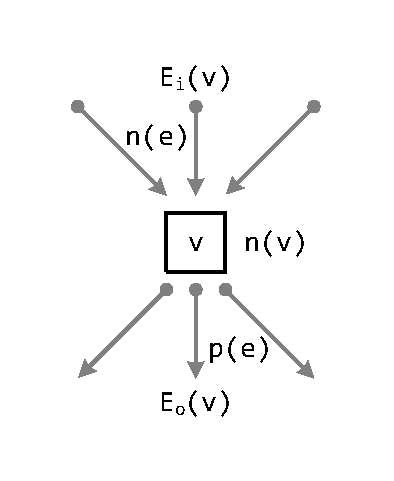
\includegraphics[width=0.4\textwidth]{./pics/text_4_flat/cfg.pdf}
\singlespacing
\captionstyle{center}\caption{Узел CFG с входящими и выходящими ребрами.}
\label{fig:text_4_vec_flat_cfg}
\end{figure}

В качестве профиля исполнения приложения будем использовать данные только счетчики узлов и ребер, а также вероятности ребер. Обозначим некоторый узел CFG через $v$.
Пусть в него входят несколько ребер, а также выходят несколько ребер (рис.~\ref{fig:text_4_vec_flat_cfg}).
Счетчиком произвольного ребра e будем называть количество переходов по этому ребру в процессе выполнения программы (значение счетчика ребра будем обозначать $n(e)$).
Счетчиком узла будем называть суммарное количество счетчиков всех входных ребер либо всех выходных ребер (для внутренних узлов CFG эти значения совпадают).
\begin{equation}
	n(v) = \sum_{e \in E_i(v)}{n(e)} = \sum_{e \in E_o(v)}{n(e)}
\end{equation}

Вероятностью ребра будем называть отношение счетчика этого ребра с счетчику узла, из которого это ребро выходит.
\begin{equation}
	\forall e \in E_o(v): p(e) = \frac{n(e)}{n(v)}
\end{equation}

Построенный по телу плоского цикла граф потока управления с собранным профилем исполнения будем использовать для принятия решения о выборе методов векторизации программного контекста.

\subsubsection{Семантика векторных инструкций AVX-512 с точки зрения понятия плоского цикла}

Векторные инструкции AVX-512 позволяют не просто объединять $w$ однотипных скалярнях операций, но также обеспечивают выборочное их исполнение с помощью векторных предикатов (масок), что делает инструкции AVX-512 мощным инструментом для векторизации плоских циклов.

В данном разделе опишем семантику некоторых векторных инструкций AVX-512, пригодных для векторизации плоских циклов.
При этом основное внимание будем уделять операциям, работающим с вещественными числами, так как обычно они являются основой высоконагруженных суперкомпьютерных приложений.
Все приводимые ниже векторные инструкции работают с упакованными данными формата float, для данных формата double в AVX-512 существуют аналогичные инструкции.

Условимся обозначать маленькими латинскими буквами элементы данных, с которыми мы оперируем в процессе счета (в данном случае это вещественные элементы данных формата float.
Арифметические операции будем записывать в естественном виде, например $r = a + b$ означает вычисление суммы двух элементов данных.
Векторы, составленные из отдельных элементов будем записывать с помощью заглавных латинских букв.
То есть будем считать, что $A$ это вектор, состоящий из $w$ отдельных элементов $A[i]$.
Под записью $R = A + B$ будем понимать поэлементную сумму векторов $A$ и $B$ и копирование результата в вектор $R$.
Заменяя операцию сложения произвольной операцией $op$ (не обязательно операцией двух аргументов), получим запись семантики векторной поэлементной операции в виде $R = op \ A, B$.

Для рассмотрения семантики векторных операций, работающих с масками, нам понадобится представление векторных предикатов.
Предикаты будем обозначать латинскими буквами в галочкой наверху.
Использование предиката при выборе одного из двух аргументов будем записывать с помощью тернарного оператора.
Таким, образом в выражении $r = \check{p} \ ? \ a : b$ элемент $r$ принимает значение $a$ при истинном значении предиката $\check{p}$, в противном случае он принимает значение $b$.
В векторном аналоге данной записи $R = \check{P} \ ? \ A : B$ эта операция выполняется поэлементно для элементов векторов, находящихся в позиции $i$ ($0 \le i < w$).

После рассмотрения записи семантики векторных инструкций для векторизации плоских циклов рассмотрим основные классы пригодных для этого инструкций (примеры операций и их семантика приведены в таблице~\ref{tbl:text_4_flat_avx512semantic}.

\begin{table}
\centering
\singlespacing
\captionstyle{center}\caption{Инструкции AVX-512 для работы с вещественными числами и их семантика.}
\bigskip
\label{tbl:text_4_flat_avx512semantic}
\begin{tabular}{ | c | c | }
  \hline
  Имя инструкции & Семантика инструкции \\ \hline\hline
  \makecell{VMOVAPS, VMOVUPS, VSQRTPS, \\ VGETEXPPS, VGETMANTPS, \\ VRCP14PS, VREDUCEPS, VRNDSCALEPS, \\ VRSQRT14PS, VSCALEFPS} & $\begin{matrix} R = op \ A \\ R = \check{P} \ ? \ (op \ A) : R \\ R = \check{P} \ ? \ (op \ A) : 0 \end{matrix}$ \\ \hline
  \makecell{VADDPS, VANDPS, VANDNPS, VDIVPS, \\ VMAXPS, VMINPS, VMULPS, VORPS, \\ VSUBPS, VRANGEPS} & $\begin{matrix} R = op \ A, B \\ R = \check{P} \ ? \ (op \ A, B) : R \\ R = \check{P} \ ? \ (op \ A, B) : 0 \end{matrix}$ \\ \hline
  \makecell{VFMADD*PS, VFMSUB*PS, \\ VFNMADD*PS, VFNMSUB*PS} & $\begin{matrix} R = op \ R, A, B \\ R = \check{P} \ ? \ (op \ R, A, B) : R \\ R = \check{P} \ ? \ (op \ R, A, B) : 0 \end{matrix}$ \\ \hline
  \makecell{VCMPPS} & $\begin{matrix} \check{P} = op \ A, B \\ \check{P} = \check{Q} \ ? \ (op \ A, B) : 0 \end{matrix}$ \\ \hline
  \makecell{VBLENDPS} & $\begin{matrix} R = \check{P} \ ? \ A : B \end{matrix}$ \\ \hline
\end{tabular}
\end{table}

Первым типом рассматриваемых операций являются векторные операции с одним аргументом.
В этом случае к каждому элементу вектора применяется одна и та же операция (например, получение обратной величины или вычисление квадратного корня), после чего результаты записываются в результирующий вектор.
С помощью дополнительного предикатного аргумента можно выбрать множество обрабатываемых элементов вектора.
Если же к элементу вектора не должна быть применена рассматриваемая операция, то соответствующий элемент результирующего вектора может быть либо оставлен без изменения, либо обнулен (это регулируется отдельным флагом в инструкци).

Аналогичным образом записывается семантика арифметических векторных инструкций с двумя и тремя аргументами.
Операции с двумя аргументами это обычные операции сложения, вычитания, умножения, получения максимума из двух чисел и другие.
Арифметические операции с тремя аргументами это так называемые сдвоенные, или комбинированные FMA операции, которые позволяют за одну операцию вычислитель значение выражения $\pm a \pm b$.

Следующий большой класс операций это операции сравнения.
В таблице данный класс представлен единственной операцией VCMPPS, однако данная операция скрывает в себе все множество различных операций сравнения (VCMPEQPS, VCMPLEPS, VCMPNEPS и остальные).
Эти операции выполняют поэлементное сравнение двух векторов и записывают результаты в векторный предикат.

Последний рассматриваемый класс векторных инструкций представлен одной инструкцией VBLENDPS, которая является реализацией векторного тернарного оператора $R = \check{P} \ ? \ A : B$.

На самом деле, глядя на таблицу~\ref{tbl:text_4_flat_avx512semantic}, можно заметить, что описания семантики всех приведенных в ней векторных операций являются просто плоскими циклами в явном виде.
Верно также и обратное -- если некий плоский цикл можно записать в виде семантики одной или нескольких векторных инструкций, то он может быть реализован с помощью этих инструкций.
